\documentclass[conference]{IEEEtran}
\IEEEoverridecommandlockouts
% The preceding line is only needed to identify funding in the first footnote. If that is unneeded, please comment it out.
\usepackage{cite}
\usepackage{amsmath,amssymb,amsfonts}
\usepackage{algorithm}
\usepackage{algorithmic}
\usepackage{graphicx}
\graphicspath{{evals/data/metrics/figures/final/}}
\usepackage{textcomp}
\usepackage{xcolor}
\usepackage{array}
\usepackage{booktabs}
\usepackage[most]{tcolorbox}

% Churkin Protocol: Color Palette (Harmonious & Minimal)
\definecolor{churkinpurple}{RGB}{94,45,121}    % #5E2D79 (for State)
\definecolor{statusgreen}{RGB}{34,139,34}      % #228B22 (Green for True - Success)
\definecolor{statusred}{RGB}{255,99,71}       % #FF6347 (Light Red/Tomato for False - Stop/Suppressed)
\def\BibTeX{{\rm B\kern-.05em{\sc i\kern-.025em b}\kern-.08em
    T\kern-.1667em\lower.7ex\hbox{E}\kern-.125emX}}

\begin{document}

\title{EXAIM: Explainable AI Middleware for Real-Time Multi-Agent Clinical Decision Support}

\author{\IEEEauthorblockN{Abem Woldesenbet}
\IEEEauthorblockA{\textit{The Beacom College of Computer \& Cyber Sciences} \\
\textit{Dakota State University}\\
Madison, SD, USA \\
abem.woldesenbet@trojans.dsu.edu}
\and
\IEEEauthorblockN{Andy Behrens}
\IEEEauthorblockA{\textit{Information Systems, College of Business \& Information Systems} \\
\textit{Dakota State University}\\
Madison, SD, USA \\
andy.behrens@dsu.edu}
}

\maketitle

\begin{abstract}
 Clinical decision support systems (CDSS) increasingly leverage multi-agent large language model (LLM) architectures to decompose complex diagnostic reasoning into specialized components. However, these systems generate verbose, interleaved reasoning traces that are difficult for clinicians to interpret in real time, limiting transparency and clinical adoption. We present EXAIM (Explainable AI Middleware), a novel middleware architecture that transforms live multi-agent reasoning traces into structured, concise summaries aligned with clinical documentation schemas. EXAIM employs a three-layer pipeline that regulates token streams, detects semantic boundaries using completeness, relevance, and novelty criteria, and generates schema-constrained summaries aligned with clinical communication frameworks (SBAR/SOAP) \cite{haig2006sbar,podder2023soap}. Unlike post-hoc explanation methods, EXAIM operates incrementally on live reasoning streams, improving information density per update while preserving diagnostic transparency. Our architecture addresses critical gaps in CDSS explainability by providing process-level narrative transparency rather than feature-importance visualizations, supporting real-time clinical workflows, and maintaining multi-agent attribution. The system's modular design enables integration with existing multi-agent CDSS frameworks while remaining agnostic to specific clinical domains or agent implementations. This work contributes a reproducible, empirically evaluated approach to explainable multi-agent clinical AI, with implications for human-AI collaboration in time-sensitive medical decision-making.
\end{abstract}

\begin{IEEEkeywords}
Clinical decision support systems, explainable artificial intelligence, multi-agent systems, large language models, real-time summarization, middleware architecture, human-AI collaboration
\end{IEEEkeywords}

\section{Introduction}

Clinical decision support systems (CDSS) increasingly employ multi-agent large language model (LLM) architectures to decompose complex diagnostic reasoning into specialized components \cite{sutton2020cdss,chenx2025diagnostic,chen2025enhancing}. While these architectures improve diagnostic performance and robustness \cite{chenx2025diagnostic,chen2025enhancing}, multi-agent systems introduce a critical usability challenge: they generate long, interleaved reasoning traces that are difficult for clinicians to interpret during time-sensitive decision-making \cite{peng2025tree,hong2024argmed,ozgun2025psychotherapy}.

Existing explainability approaches are misaligned with real-time clinical workflows and fail to adequately address cognitive load in clinical settings \cite{hor2025design,abbas2025xai}. Current multi-agent interfaces surface outputs at turn boundaries, but LLM turns often contain multiple topic shifts and incomplete reasoning, creating lossy compression when summarized. This motivates semantic event detection that triggers updates based on content completeness rather than generation structure.

To address these challenges, we propose EXAIM (Explainable AI Middleware), a real-time summarization architecture designed to bridge the gap between multi-agent reasoning complexity and clinical information needs. The following research question guides this work:

\textbf{RQ1:} Can event-driven, schema-constrained summarization improve trace utility by increasing semantic coverage while reducing redundant updates?

Following a design science research paradigm, RQ1 is investigated through the construction and evaluation of a summarization middleware artifact. The research question is operationalized via four sub-questions, each corresponding to a distinct evaluation dimension of the artifact:

\begin{itemize}
\item \textbf{RQ1a:} Does EXAIM improve global semantic trace coverage under identical schema and length constraints?
\item \textbf{RQ1b:} Does EXAIM reduce redundant and low-novelty updates through semantic buffering and novelty filtering?
\item \textbf{RQ1c:} Does EXAIM preserve contract-grounded faithfulness when limited continuity across summaries is permitted?
\item \textbf{RQ1d:} What impact does semantic event detection introduce relative to simpler triggers such as turn boundaries or fixed-interval chunking?
\end{itemize}

To evaluate these questions, we conducted an ablation study in which we instantiated a real-time summarization middleware that intercepts LLM reasoning traces and emits structured summaries constrained by a fixed schema. The artifact enables controlled variation of triggering strategies (event-driven versus baseline triggers), continuity constraints, and update policies, allowing systematic assessment of their effects on semantic coverage, redundancy, faithfulness, and computational overhead.

This paper makes the following contributions:
\begin{itemize}
\item \textbf{A modular middleware architecture that transforms streaming multi-agent reasoning traces into structured, clinician-aligned summaries.}
\item \textbf{A semantic buffering mechanism that detects topic shifts, novelty, and critical clinical events to trigger summaries based on context.}
\item \textbf{Development of process-level transparency through structured summaries aligned with SBAR/SOAP communication patterns, preserving agent attribution and uncertainty while enforcing strict brevity constraints.}
\item \textbf{Identification of the impact of semantic buffering on coverage, redundancy, faithfulness, and computational cost in clinical reasoning streams.}
\end{itemize}

The remainder of this paper is organized as follows. Section II provides a comprehensive review of related work in clinical decision support explainability, multi-agent architectures, streaming interfaces, and clinical summarization, establishing the technical foundations and identifying gaps that motivate our approach. Section III provides a systematic description of the EXAIM artifact, including its architecture, component specifications, and design rationale. Section IV presents the experimental design, ablation study, and evaluation results. Section V discusses key findings and implications for clinical AI system design. Section VI concludes with limitations and future directions.

\section{Literature Review}
\subsection{Clinical Decision Support Systems and Explainability}
Clinical decision support systems (CDSS) have demonstrated potential to improve diagnostic accuracy and patient safety \cite{sutton2020cdss,miyachi2023learning}, yet their real-world adoption remains constrained by usability and workflow integration challenges \cite{derksen2025cdss,bayor2025cdss,harrison2022patient}. Prior studies emphasize that excessive alerting, poor timing, and opaque system behavior contribute to clinician frustration and alert fatigue, limiting trust and sustained use \cite{marcilly2018alerts}. As CDSS increasingly incorporate machine learning and large language models (LLMs), explainability has emerged as a critical requirement for safe deployment in clinical environments \cite{abbas2025xai,chen2025enhancing,hong2024argmed,salimiparsa2021design,sutton2020cdss}. A recent systematic review of CDSS design emphasizes that effective systems must balance clinical accuracy with usability, integration, and transparency \cite{bayor2025cdss}.

\subsubsection{Post-Hoc XAI Methods and Their Limitations}
Explainable AI (XAI) approaches in CDSS have largely focused on post-hoc interpretation methods. Feature importance techniques, including LIME and SHAP, generate local explanations by perturbing inputs and measuring output sensitivity \cite{abbas2025xai,salimiparsa2021design}. Gradient-based visualization methods, such as GradCAM, highlight salient input regions influencing predictions \cite{goel2022covid}. Surrogate model approaches approximate complex models with interpretable alternatives \cite{ribeiro2016lime,guidotti2018survey}.

Frameworks for evaluating XAI systems emphasize the importance of both technical performance and user-centered criteria, suggesting that effective explainability requires consideration of information presentation, cognitive load, and task alignment \cite{vilone2021explainable}. However, these post-hoc methods face critical limitations in real-time clinical workflows. They are poorly aligned with time-sensitive decision-making \cite{abbas2025xai,salimiparsa2021design}, exposing internal model mechanics rather than the evolving clinical narrative \cite{benzion2025anxiety,salimiparsa2021design,hong2024argmed}.

\subsubsection{Cognitive Load and Information Overload}
Traditional explainability approaches fail to account for distributed reasoning and high-velocity, redundant trace emissions that increase output volume and cognitive overload in clinicians \cite{sanwal2025layered,hong2024argmed}. Recent work emphasizes that AI systems for general practice must address cognitive load through transparency that supports clinical sensemaking rather than exposing internal model mechanics \cite{hor2025design}. The update frequency in clinician-facing interfaces often results in verbose or redundant information that does not reflect the summarized treatment plan \cite{wu2025incremental}.

\subsubsection{Clinician Preference for Narrative Explanations}
Empirical studies show that clinicians often prefer concise, narrative explanations grounded in clinical reasoning over probabilistic or feature-based explanations in time-sensitive contexts \cite{silva2023xai}. This misalignment between existing XAI techniques and clinical information needs motivates alternative approaches to explainability that prioritize process transparency and clinical understanding \cite{abbas2025xai,schoonderwoerd2021patterns,salimiparsa2021design,hong2024argmed,derksen2025cdss}. While XAI methods address model interpretability challenges, multi-agent architectures introduce additional complexity in distributing and coordinating explainable reasoning across specialized components.

\subsection{Multi-Agent Systems for Clinical Reasoning}
Multi-agent LLM architectures have gained traction as a means of decomposing complex clinical reasoning tasks across specialized agents responsible for information retrieval, hypothesis generation, verification, and safety assessment \cite{hong2024argmed,ozgun2025psychotherapy,chen2025enhancing}. Prior work demonstrates that distributing reasoning across agents can improve diagnostic performance, robustness, and oversight compared to monolithic models \cite{chenx2025diagnostic,chen2025enhancing,hong2024argmed,peng2025tree}. These systems also offer theoretical advantages for transparency, as individual agents can be assigned interpretable roles within the diagnostic process \cite{ozgun2025psychotherapy}. However, multi-agent systems introduce new explainability challenges. Agent interactions generate long, interleaved reasoning traces that include exploratory hypotheses, internal deliberation, and repetitive grounding statements \cite{hong2024argmed}. While some systems explicitly expose agent reasoning to users, these traces are typically verbose and require post-hoc review, limiting their practical utility during live clinical decision-making. Existing multi-agent frameworks largely assume that transparency is achieved by exposing reasoning in full, rather than by managing how and when information is presented to clinicians \cite{wu2025incremental,leduc2025speech,schneider2024meeting}. The verbosity of multi-agent reasoning traces is compounded by interface design choices, particularly turn-based interaction paradigms that misalign with semantic completeness.

\subsection{Turn-Based Interfaces and Streaming Reasoning}

\subsubsection{Limitations of Turn-Based Paradigms}
Most conversational and multi-agent AI systems adopt turn-based interaction paradigms, surfacing outputs only when an agent completes a turn. This abstraction is inherited from human dialogue systems, where turn-taking often corresponds to semantic completion. However, in multi-agent LLM systems, a single turn may contain multiple topic shifts, partial inferences, or exploratory reasoning branches. Treating turns as semantic units can therefore result in lossy compression, redundancy, and reduced faithfulness when summarization is applied. When multi-agent reasoning traces are compressed at turn boundaries, semantically incomplete fragments may be forced into summaries, while complete reasoning spans crossing turn boundaries may be artificially split. This leads to information loss, as partial hypotheses and exploratory statements are either omitted or presented without sufficient context.

\subsubsection{Semantic Boundary Detection in Streaming Systems}
Recent work on streaming and incremental reasoning highlights the limitations of turn-based interfaces in high-velocity information environments \cite{leduc2025speech,wu2025incremental}. Studies in meeting summarization demonstrate that incremental updates triggered by semantic boundaries rather than fixed intervals improve information retention and regularize update frequency \cite{schneider2024meeting}. Similar findings emerge in customer support and medical dialogue systems, where content-based triggering outperforms interval-based approaches. These findings suggest that real-time systems require adaptive mechanisms to regulate information flow based on content semantics rather than generation structure. For multi-agent clinical decision support, this implies that summarization triggers should be driven by semantic completeness, clinical relevance, and novelty rather than arbitrary turn boundaries or fixed time intervals.

Addressing these interface challenges requires not only semantic event detection but also structured presentation formats aligned with clinical communication practices and documentation standards.



\subsection{Clinical Summarization and Structured Communication}
Clinical summarization research provides important foundations for managing information overload in healthcare settings \cite{vanveen2023summarization,leduc2025speech,yim2023acibench,krishna2021soap}.

\subsubsection{Clinical Communication Frameworks}
Structured summaries aligned with clinical documentation standards, such as SBAR (Situation-Background-Assessment-Recommendation) and SOAP (Subjective-Objective-Assessment-Plan), support predictable, scannable presentation formats \cite{haig2006sbar,podder2023soap}. These frameworks reduce communication errors and support clinical handoff processes \cite{krishna2021soap,zhang2024annotate}. The SBAR framework structures information into four components: current situation, relevant background context, clinical assessment, and recommended actions. SOAP notes organize clinical encounters into subjective patient reports, objective measurements, diagnostic assessment, and treatment plans. Both frameworks emphasize brevity, actionability, and role-appropriate information density.

\subsubsection{LLM-Based Clinical Summarization}
Large language models have shown strong performance in generating clinical summaries when explicit length and structure constraints are enforced \cite{vanveen2023summarization}. Recent work on LLM-based clinical dialogue summarization has validated the use of expert clinician evaluation for assessing summary quality, emphasizing faithfulness, completeness, and clinical utility as key evaluation criteria \cite{fraile2025llm}.

\subsubsection{Streaming and Real-Time Summarization}
Recent studies indicate that streaming summarization can outperform post-hoc summarization by preserving context and reducing the need for retrospective compression \cite{bailly2025divide}. Additionally, token filtering strategies have been proposed to reduce redundancy in clinical texts \cite{piya2025contextual}. However, most clinical summarization systems operate on completed conversations or documents and do not address the challenges posed by multi-agent reasoning streams \cite{wu2025incremental,schneider2024meeting}. Specifically, they assume a single narrative source rather than multiple interacting agents producing overlapping and partially redundant content. Human-in-the-loop dialogue systems literature emphasizes the importance of faithfulness and coherence as critical evaluation dimensions for interactive systems \cite{chen2022hitl}. To our knowledge, prior systems do not jointly perform semantic event triggering over interleaved multi-agent traces and emit clinician-aligned schema summaries. EXAIM integrates concepts from XAI, clinical summarization, and streaming systems by introducing a dedicated middleware layer that regulates information flow, detects meaningful reasoning events, and generates clinician-aligned summaries in real time. % Added positioning statement

\section{Artifact Description}

Design Science aims to create and evaluate IT artifacts intended to solve identified organizational problems \cite{hevner2004design}. We adhere to the six design steps of DSR and the nominal process model outlined by Peffers et al. \cite{peffers2007dsr} in designing EXAIM (Figure~\ref{fig:dsr}). This approach aligns with recent applications of DSR for developing AI-based clinical tools that balance technical innovation with practical usability requirements \cite{hor2025design}. This section systematically provides a comprehensive description of the artifact design, EXAIM.

\begin{figure*}[htbp]
\centering
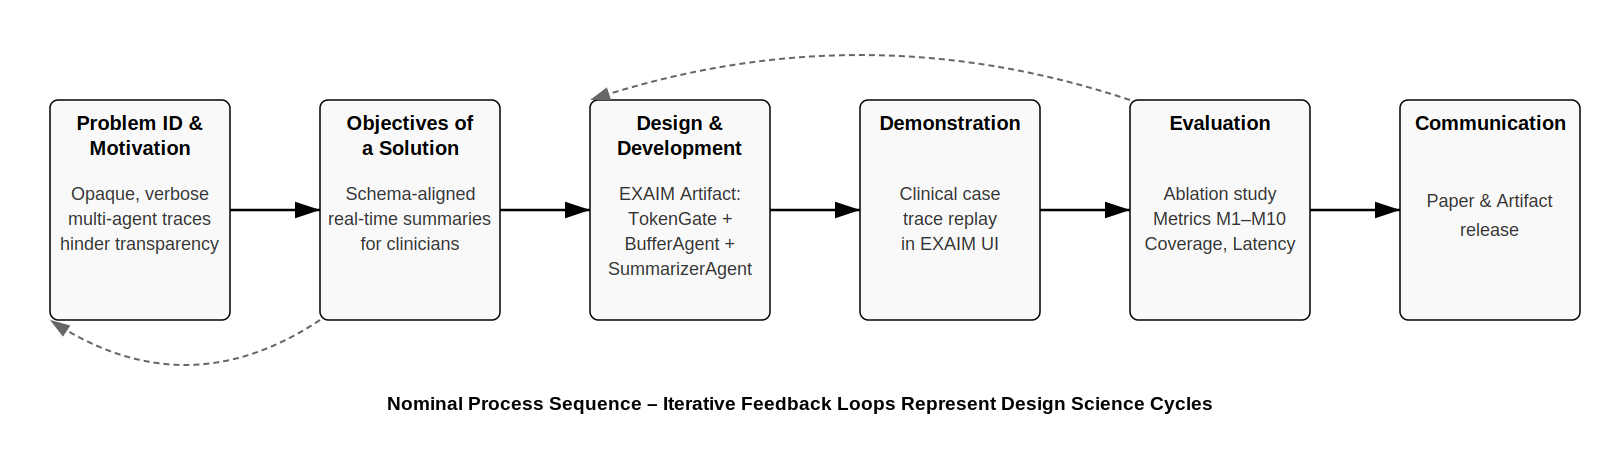
\includegraphics[width=\textwidth]{dsr/DSR.pdf}
\caption{EXAIM Design Science Research Methodology (DSRM) process model showing the six stages of our research lifecycle and the process iteration feedback loops.}
\label{fig:dsr}
\end{figure*}

\subsection{EXAIM Architecture Overview}

Building on recent advances in incremental summarization \cite{leduc2025speech,wu2025incremental}, EXAIM operates as an intermediary layer between upstream diagnostic agents and clinician-facing interfaces, continuously monitoring reasoning streams and generating concise, structured summaries at clinically meaningful moments. Rather than relying on fixed turn boundaries or static thresholds, the system employs semantic event detection to trigger updates only when new, relevant, and non-redundant clinical information emerges.

Figure~\ref{fig:system-architecture} illustrates EXAIM's three-stage transformation pipeline. The architecture is implemented as a modular, domain-agnostic middleware composed of three specialized components: (i) \textbf{TokenGate}, a syntax-aware stream regulator that segments high-velocity token streams into semantically coherent units, (ii) \textbf{BufferAgent}, a semantic buffering agent that detects topic shifts, novelty, and critical events, and (iii) \textbf{SummarizerAgent}, a schema-constrained summarization agent that produces structured updates aligned with established clinical communication frameworks (SBAR/SOAP).

This design supports incremental transparency by progressively transforming raw token streams into structured summaries. The architecture controls update stream quality through semantic event detection and novelty filtering, suppressing redundant or low-value updates while preserving multi-agent attribution. Importantly, EXAIM operates without requiring modification of upstream diagnostic models, functioning purely as an observational transparency layer. The approach leverages evidence that strict length constraints and structured documentation \cite{haig2006sbar,podder2023soap} support predictable, scannable presentation formats in clinical communication \cite{vanveen2023summarization,krishna2021soap,zhang2024annotate}.

The three-stage pipeline operates as follows: First, TokenGate accumulates per-agent text deltas and flushes chunks when syntax-aware conditions are met (word thresholds, sentence boundaries, or timeouts). Second, BufferAgent analyzes each flushed chunk for semantic properties—completeness, relevance, and novelty—deciding whether to trigger summarization. Third, when triggered, SummarizerAgent generates a schema-constrained summary that enforces character limits and clinical framework alignment. This staged design decouples stream regulation (syntactic), event detection (semantic), and summary generation (structural), enabling independent tuning and ablation of each component. Sections 3.B--3.D detail the implementation of each component, while Section 3.E specifies the output schema and Section 3.F demonstrates the system's filtering behavior through a case walkthrough.

\subsubsection{Interface Model}

EXAIM processes asynchronous streams of text deltas and emits structured summaries at semantically detected events. The system assumes a stream-based input model where multiple upstream agents emit incremental text deltas asynchronously. Each delta is a tuple $(a, \tau)$ where $a$ is the agent identifier and $\tau$ is a text fragment (substring of ongoing generation). The middleware subscribes to this stream via callback registration, operating in push mode without blocking upstream generation. Timing information is inferred from arrival timestamps rather than explicit metadata, allowing integration with any agent framework supporting token-level streaming.

\subsubsection{Output Contract}

EXAIM emits structured summaries conforming to a fixed six-field schema with hard character limits totaling 990 characters. The schema enforces alignment with SBAR \cite{haig2006sbar} and SOAP \cite{podder2023soap} clinical communication patterns:
\begin{itemize}
\item \textbf{status\_action} (150 chars): Current diagnostic activity (SBAR: Situation)
\item \textbf{key\_findings} (180 chars): Salient clinical evidence (SOAP: Subjective/Objective)
\item \textbf{differential\_rationale} (210 chars): Diagnostic interpretation (SOAP: Assessment)
\item \textbf{uncertainty\_confidence} (120 chars): Confidence signals
\item \textbf{recommendation\_next\_step} (180 chars): Actionable plan (SBAR: Recommendation / SOAP: Plan)
\item \textbf{agent\_contributions} (150 chars): Multi-agent attribution metadata
\end{itemize}

This bounded schema serves as a UI contract, guaranteeing stable interface footprint regardless of trace verbosity—a key requirement for real-time clinical dashboards.

\begin{figure*}[htbp]
    \centering
    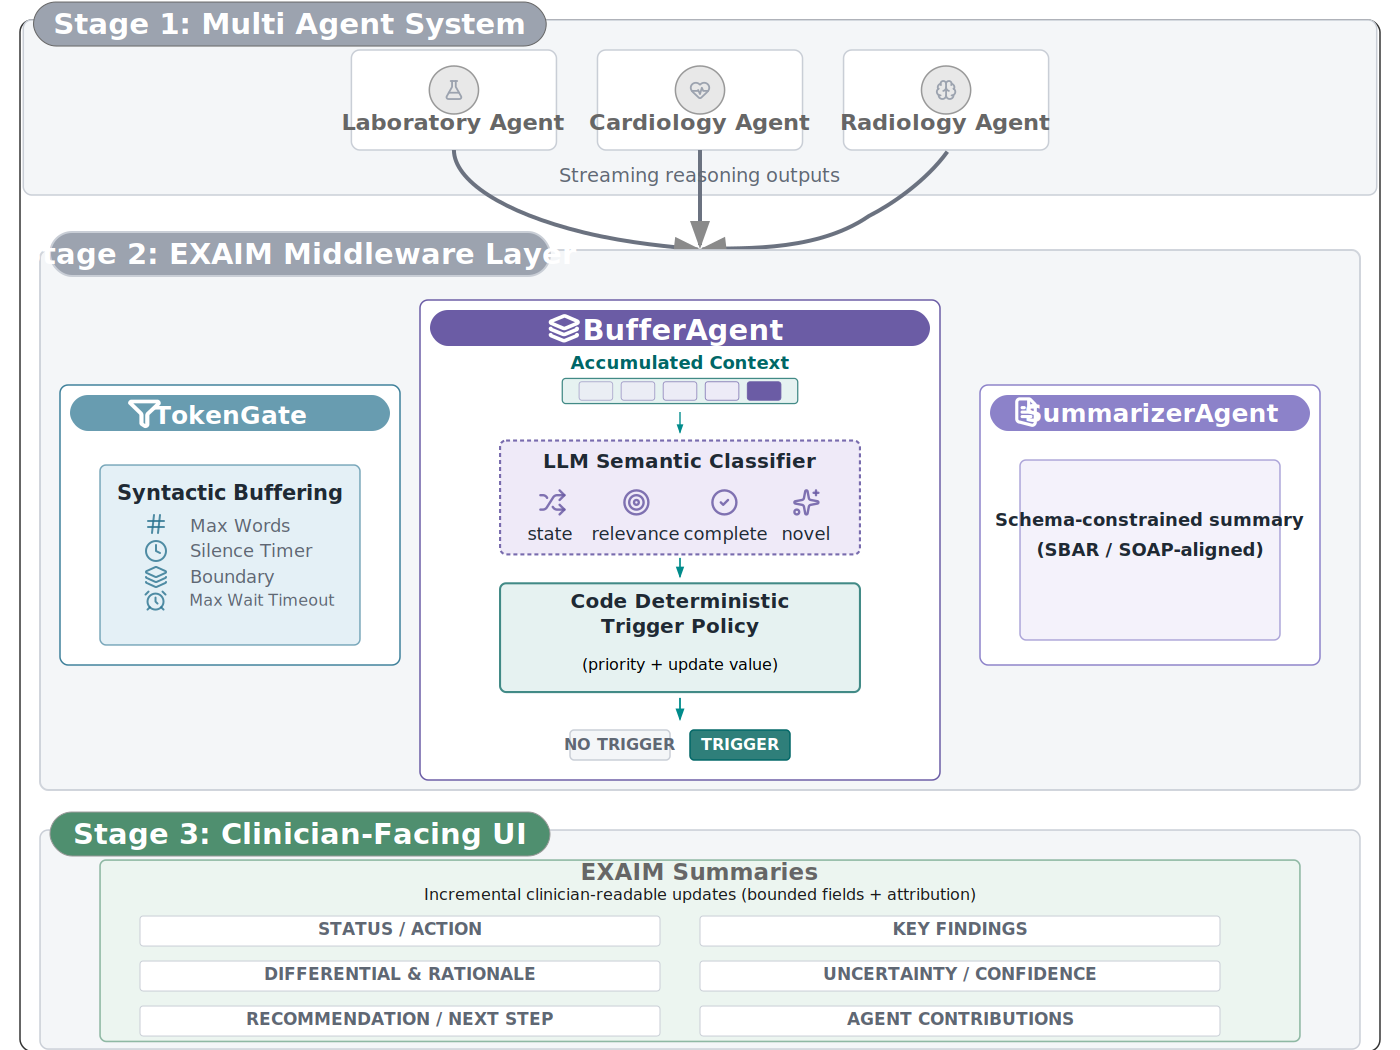
\includegraphics[width=\textwidth]{../raw/systemFigure/system.pdf}
    \caption{EXAIM System Architecture Overview showing the three-stage pipeline: (1) Stage 1: Interleaved Input Stream from external agents (Laboratory, Cardiology, Radiology), (2) Stage 2: EXAIM Middleware Layer with TokenGate (syntax-aware buffering), BufferAgent (semantic boundary detection), and SummarizerAgent (schema-constrained compression), and (3) Stage 3: Structured Output in SBAR/SOAP format. The diagram illustrates the flow of streaming token deltas through the middleware, semantic event detection, and the generation of coherent, bounded summaries for clinician-facing interfaces.}
    \label{fig:system-architecture}
\end{figure*}

\subsubsection{System Assumptions and Constraints}

The architecture enforces three core constraints:
\begin{itemize}
\item \textbf{Non-Blocking Observation}: Middleware processing occurs asynchronously without delaying upstream agent generation
\item \textbf{Schema Compliance}: All emitted outputs conform to the AgentSummary schema or are marked as validation failures
\item \textbf{Grounding Constraint}: Summary generation is restricted to buffered trace content and limited prior context (history\_k=3). No external retrieval or extrapolation beyond observed agent outputs is permitted
\end{itemize}

These constraints operationalize the middleware's role as a transparency layer rather than an autonomous reasoning component.

\subsection{TokenGate: Syntax-Aware Stream Regulation}

TokenGate addresses a fundamental problem in streaming LLM interfaces: raw token streams are fragmented, bursty, and misaligned with linguistic boundaries. Applying semantic analysis directly to these streams would either trigger excessive processing on partial phrases or buffer indefinitely on incomplete units. TokenGate solves this by accumulating text deltas into coherent chunks using a syntax-aware segmentation policy.

To maintain low latency and avoid dependencies on model-specific tokenizers (e.g., BPE, TikToken), TokenGate operates on whitespace-delimited word counts rather than subword tokens. This design choice trades fine-grained precision for computational simplicity and cross-model portability.

\subsubsection{Segmentation Policy}

TokenGate accumulates per-agent text deltas and emits chunks under a prioritized four-clause policy designed to balance latency, linguistic coherence, and computational efficiency:

\begin{enumerate}
\item \textbf{Boundary-Aware}: Flush when word count $\geq$ 60 AND text ends with sentence-final punctuation (\texttt{[.?!]})
\item \textbf{Hard Limit}: Flush when word count $>$ 100 regardless of boundary status
\item \textbf{Silence Timeout}: Flush after 1.0s idle time if word count $\geq$ 60
\item \textbf{Safety Valve}: Force flush after 4.0s total accumulation time regardless of other conditions
\end{enumerate}

This policy prioritizes sentence boundaries when available (clause 1) but prevents indefinite blocking through hard limits (clauses 2-4). The design avoids dependencies on model-specific tokenizers by operating on whitespace-delimited word counts, ensuring portability across LLM providers.

\subsubsection{Design Rationale and Ablation}

Clause 1 implements adaptive boundary detection, allowing chunks to align with semantic units. Ablation variant V3 (Fixed-Chunk) disables this adaptivity by removing the boundary condition. This isolates the impact of syntax-aware segmentation on downstream semantic coverage. Parameter values (60/100 words, 1.0s/4.0s timeouts) were calibrated through Pareto optimization across 625 configurations (Section IV-A), balancing first-chunk latency, semantic coherence, and processing overhead.

\subsection{BufferAgent: Semantic Event Detection}

BufferAgent implements the core innovation of EXAIM: event-driven triggering based on content semantics rather than generation mechanics. This component operationalizes RQ1b (reducing redundant updates) and RQ1d (comparing semantic versus structural triggers) by detecting when buffered content represents a clinically meaningful update.

\subsubsection{Semantic Evaluation Predicates}

The system evaluates each flushed chunk using an LLM-based semantic classifier that produces four boolean predicates:

\begin{enumerate}
\item $\mathit{complete}$: Chunk exhibits phrase-level structural closure (finished clause, action statement, or sentence boundary)
\item $\mathit{relevant}$: Content contributes interruption-worthy clinical value (diagnostic shifts, abnormal findings, or action changes)
\item $\mathit{novel}$: Content introduces substantive information not already captured in recent summaries (history\_k=3)
\item $\mathit{state} \in \{\text{CONTINUING}, \text{SHIFT}, \text{CRITICAL}\}$: Topic continuity classification
\end{enumerate}

Crucially, novelty is assessed against prior \textit{summaries} rather than raw trace content, preventing redundancy at the output level where it impacts clinician cognitive load.

\subsubsection{Multi-Path Trigger Function}

The trigger decision follows a three-path logic that balances urgency, topic boundaries, and content quality:

\[
\mathit{trigger} = \begin{cases}
\mathit{true} & \text{if } \mathit{state} = \text{CRITICAL} \\
\mathit{true} & \text{if } \mathit{complete} \land \mathit{relevant} \land \mathit{novel} \\
\mathit{true} & \text{if } (\mathit{state} = \text{SHIFT}) \land \mathit{relevant} \land \mathit{novel} \\
\mathit{false} & \text{otherwise}
\end{cases}
\]

Path 1 (critical alerts) bypasses all filtering for urgent events. Path 2 (complete value) requires full semantic and structural criteria. Path 3 (topic shift) relaxes the completeness requirement at topic boundaries, enabling responsive updates when diagnostic focus changes. This prioritization addresses a key limitation of turn-based or fixed-interval approaches: they cannot distinguish between incremental elaboration and substantive topic transitions.

\subsubsection{Ablation Points}

The multi-path design enables targeted ablations:
\begin{itemize}
\item \textbf{V4 (No Novelty)}: Forces $\mathit{novel} = \mathit{true}$, isolating novelty filtering's impact on redundancy
\item \textbf{V1 (Turn-End)}: Bypasses semantic evaluation entirely, triggering on agent turn boundaries
\item \textbf{V2 (No BufferAgent)}: Removes semantic layer, processing all TokenGate chunks
\end{itemize}

These variants directly test the contribution of semantic event detection to coverage (RQ1a), redundancy (RQ1b), and comparative performance (RQ1d).

\subsection{SummarizerAgent: Schema-Constrained Synthesis}

SummarizerAgent generates structured clinical summaries conforming to the AgentSummary schema. This component enforces strict character limits, maintains SBAR/SOAP alignment, and implements grounding constraints to prevent hallucination.

\subsubsection{Schema and Character Budgets}

Table~\ref{tab:schema} details the six-field schema with evidence-based character limits. These limits operationalize qualitative usability principles (``brief titles,'' ``short snippets'') \cite{pourian2025alerts,vanveen2023summarization} into deterministic constraints. Character budgets function as a bounded UI contract, ensuring stable interface footprint regardless of model verbosity.

\subsubsection{Grounding Strategy}

The summarizer operates under strict grounding rules:
\begin{itemize}
\item \textbf{PRIMARY SOURCE}: Current buffered chunk (new information to summarize)
\item \textbf{SECONDARY SOURCE}: Latest summary from history (for continuity only, history\_k=3)
\item \textbf{PROHIBITED}: External knowledge, speculation, or extrapolation beyond provided context
\end{itemize}

If a field has no new information, the summary must reflect this absence through explicit placeholder text (e.g., ``No new findings'') rather than repeating prior content or inventing information.

\subsubsection{Validation and Fallback Strategy}

Schema compliance is enforced through a three-attempt strategy:
\begin{enumerate}
\item \textbf{Initial Generation}: Structured output with Pydantic schema (strict=True)
\item \textbf{Retry with Rewrite}: If character limits exceeded, prompt model to condense specific fields
\item \textbf{Truncation Fallback}: If validation still fails, apply hard truncation at character boundaries
\end{enumerate}

Failed summaries (after all attempts) are logged with schema\_ok=false and excluded from metrics, but the system continues operation to maintain availability.

\subsubsection{Implementation Details}

\begin{itemize}
\item \textbf{Input}: Text chunk, summary history (last 3), agent\_id
\item \textbf{Output}: AgentSummary (6 fields, total $\leq$990 characters)
\item \textbf{Validation}: Three-attempt strategy (structured generation $\rightarrow$ rewrite prompt $\rightarrow$ truncation fallback)
\item \textbf{LLM Configuration}: Structured output mode with schema enforcement (Pydantic strict mode). Model selection and sampling parameters detailed in Section IV-A
\end{itemize}

\subsection{Schema Specification}

The AgentSummary schema (Table~\ref{tab:schema}) enforces a structured contract between the middleware and clinician-facing interfaces. Each of the six fields maps directly to elements of SBAR (Situation-Background-Assessment-Recommendation) \cite{haig2006sbar} and SOAP (Subjective-Objective-Assessment-Plan) \cite{podder2023soap} clinical communication frameworks. Character budgets operationalize qualitative usability principles from clinical alert systems \cite{pourian2025alerts} and patient-centered CDSS design \cite{harrison2022patient} into deterministic constraints.

The schema design reflects three core principles: (1) \textit{Scannability}: Brief field lengths force summarization to salient points, preventing verbose blocks that impair rapid comprehension. (2) \textit{Clinical Alignment}: Field semantics mirror established documentation workflows, reducing cognitive overhead for clinician users. (3) \textit{Bounded Contracts}: Hard character limits guarantee stable UI footprint regardless of model verbosity, preventing layout shifts or overflow in dashboard interfaces.

\begin{table*}[htbp]
\caption{EXAIM Summary Schema: Clinical Mapping and Bounded Output Budgets}
\label{tab:schema}
\begin{center}
\renewcommand{\arraystretch}{1.3}
\begin{tabular}{p{2.5cm}p{2.5cm}p{4cm}p{1.5cm}p{4.5cm}}
\toprule
\textbf{Field} & \textbf{Clinical Map} & \textbf{Role} & \textbf{Budget (Chars)} & \textbf{Design Motivation} \\
\midrule
Status / Action & SBAR: Situation & Alert header; scannable update. & 150 chars & Enforces scannability via brief title heuristic \cite{pourian2025alerts}. \\
Key Findings & SOAP: Obj/Subj & Salient facts; ``live snippet'' paradigm. & 180 chars & Supports $\sim$2 concise snippets aligned with targeted summarization limits \cite{vanveen2023summarization}. Structured presentation addresses transparency barriers identified in patient-centered CDSS deployment \cite{harrison2022patient}. \\
Differential & SOAP: Assessment & Diagnostic interpretation. & 210 chars & Bounds complexity to maintain interpretability \cite{lage2019interpretability}. \\
Uncertainty & SOAP: Assessment & Explicit confidence signal. & 120 chars & Simplified framing for trust calibration \cite{goel2022covid}. \\
Rec. / Plan & SOAP: Plan & Actionable next step. & 180 chars & Action-linked explanations \cite{silva2023xai}. \\
Agent Contrib. & System Meta & Attribution of active agents. & 150 chars & Pipeline transparency patterns \cite{donadello2021sexai}. \\
\bottomrule
\end{tabular}
\end{center}
\footnotesize
Note: Character budgets are hard constraints that enforce a bounded UI contract, ensuring stable interface footprint regardless of model verbosity.
\normalsize
\end{table*}

\subsection{Demonstrative Case Walkthrough}

To demonstrate EXAIM's semantic filtering and redundancy detection mechanisms, we analyze a specific interaction sequence from a multi-agent reasoning trace (Case ID: 3949). This trace was generated using the MAC Framework (described in Section IV-A), which simulates a team of diagnostic agents collaborating on a complex medical case. This example illustrates how the middleware distinguishes between verbose repetition and genuinely novel clinical information.

\textbf{1. Context State (Pre-Condition)} Prior to this segment, doctor0 and doctor1 had already established Spinocerebellar Ataxia (SCA) as the leading diagnosis. The middleware had generated summaries capturing this consensus and the recommended genetic tests (Log ID: summary\_3). The active buffer was empty.

\textbf{2. The Raw Input Stream} doctor2 then enters the discussion. The agent generates a verbose response concurring with the previous agents and re-stating the established diagnosis.

\textit{Raw Trace (doctor2):} ``\textit{\#\#\# Most Likely Diagnosis: Spinocerebellar Ataxia (SCA): I concur with both Doctor0 and Doctor1 that the most likely diagnosis is spinocerebellar ataxia... The gradual onset at age 30 years also aligns with hereditary SCAs... \#\#\# Differential Diagnoses: 1. Multiple Systems Atrophy (MSA): While I agree that MSA typically presents with...}''

\textbf{3. BufferAgent Logic (Internal Rationale)} While the dashboard remained visually static (see Fig.~\ref{fig:suppression-demo}), the middleware was actively analyzing the stream. As visualized in Fig.~\ref{fig:logic-card}, the system detected semantic redundancy through its multi-stage evaluation process. Despite the input's clinical relevance, the novelty check failed, causing the middleware to suppress the update and prevent redundancy.

\begin{figure}[h]
    \centering
    \scalebox{0.75}{%
    \begin{tcolorbox}[
        enhanced,
        colback=white,
        colframe=black,
        boxrule=0.5mm,
        arc=2mm,
        drop shadow,
        left=4mm,
        right=4mm,
        top=2mm,
        bottom=2mm,
        title=\textbf{BufferAgent Status [doctor2]},
        fonttitle=\bfseries\normalsize,
        coltitle=black,
        colbacktitle=white,
        halign title=center,
        fontupper=\normalsize
    ]
        \normalsize
        
        \textbf{Input Stream:}
        \vspace{-1mm}
        \begin{quote}
            \itshape "...I concur with both Doctor0 and Doctor1... adding no new information."
        \end{quote}
        \vspace{1.5mm}
        
        \textbf{Decision Flags:}
        \vspace{0.5mm}
        
        \begin{center}
        \begin{tabular}{@{}c@{}}
            \raisebox{5pt}{State} \\
            \tcbox[colback=churkinpurple!15, colframe=churkinpurple, size=small, boxrule=0.5mm, left=2mm, right=2mm, top=0.5mm, bottom=0.5mm, fontupper=\normalsize]{\textcolor{churkinpurple}{\texttt{SAME\_TOPIC\_CONTINUING}}}
        \end{tabular}
        \end{center}
        
        \vspace{0.1mm}
        \begin{center}
        \begin{tabular}{@{}c@{\hspace{2mm}}c@{\hspace{2mm}}c@{}}
            \begin{tabular}{@{}c@{}}
                \raisebox{5pt}{Complete} \\[-3pt]
                \tcbox[colback=statusgreen!15, colframe=statusgreen, size=small, boxrule=0.5mm, left=2mm, right=2mm, top=0.2mm, bottom=0.2mm, fontupper=\normalsize]{\textcolor{statusgreen}{\textbf{True}}}
            \end{tabular} &
            \begin{tabular}{@{}c@{}}
                \raisebox{5pt}{Relevant} \\[-3pt]
                \tcbox[colback=statusgreen!15, colframe=statusgreen, size=small, boxrule=0.5mm, left=2mm, right=2mm, top=0.2mm, bottom=0.2mm, fontupper=\normalsize]{\textcolor{statusgreen}{\textbf{True}}}
            \end{tabular} &
            \begin{tabular}{@{}c@{}}
                \raisebox{5pt}{Novel} \\[-3pt]
                \tcbox[colback=statusred!15, colframe=statusred, size=small, boxrule=0.5mm, left=2mm, right=2mm, top=0.2mm, bottom=0.2mm, fontupper=\normalsize]{\textcolor{statusred}{\textbf{False}}}
            \end{tabular} \\
        \end{tabular}
        \end{center}
        \vspace{-2mm}
        \begin{center}
            $\downarrow$
        \end{center}
        \vspace{-2mm}
        \begin{center}
            \tcbox[
                enhanced,
                colback=statusred!20,
                colframe=statusred,
                boxrule=0.5mm,
                size=normal,
                fontupper=\bfseries\normalsize,
                left=3mm,
                right=3mm,
                top=0.5mm,
                bottom=0.5mm
            ]{\textcolor{statusred}{Trigger = False (Suppressed)}}
        \end{center}
        
        \vspace{0.1mm}
        \noindent\rule{\linewidth}{0.5mm}
        \vspace{0.5mm}
        
        \textbf{Rationale:} Doctor2 concurs with SCA based on ataxia/dysarthria/MRI... adding no new information. The content is \textcolor{statusgreen}{relevant} as it details planned actions, but it is \textcolor{statusred}{not novel} as these details were already broadly mentioned in previous summaries.
    \end{tcolorbox}%
    }
    \caption{BufferAgent System Status Card showing the hierarchical decision logic. Three evaluation conditions (\textcolor{statusgreen}{Complete=True}, \textcolor{statusgreen}{Relevant=True}, \textcolor{statusred}{Novel=False}) combine to produce the final result: \textcolor{statusred}{Trigger=False (Suppressed)}, preventing redundant update generation.}
    \label{fig:logic-card}
\end{figure}

\begin{figure*}[htbp]
\centering
\includegraphics[width=\textwidth]{case_walkthrough/CaseWalkthroughImage.png}
\caption{The EXAIM dashboard during redundancy suppression. The left panel shows the raw, verbose stream from doctor2 concurring with the diagnosis. The right panel remains static (displaying the previous doctor1 update), visually confirming that the middleware successfully filtered the non-novel content.}
\label{fig:suppression-demo}
\end{figure*}

\textbf{4. Outcome} Consequently, EXAIM filtered this update, preventing the generation of a low-value summary. The middleware continued to buffer doctor2's subsequent tokens silently until the agent introduced specific new details regarding ``High-Resolution MRI techniques'' and ``Oligoclonal bands,'' which finally triggered a consolidated, high-density update.

\section{Experiments and Results}

To isolate the architectural contribution of EXAIM, we employ a ``glass-box'' evaluation methodology using deterministic replays of multi-agent reasoning traces. This approach allows us to stress-test the middleware's flow-control capabilities independent of variations in upstream agent behavior. The evaluation employs automated metrics to enable reproducible, systematic comparison across variants, aligning with established frameworks for XAI evaluation that emphasize both technical performance and user-centered criteria \cite{vilone2021explainable}.

\subsection{Experimental Setting}

\subsubsection{Upstream Trace Generation}

To evaluate the EXAIM middleware, we utilized the Multi-Agent Conversation (MAC) framework \cite{chenx2025diagnostic} as the upstream trace generator. MAC is a multi-agent diagnostic system where diverse doctor agents and a supervisor collaborate to solve complex medical cases.

For this study, we instrumented the MAC framework to capture the real-time dynamics of these multi-agent interactions. Specifically, we modified the upstream codebase to log granular stream deltas (chunk-level text outputs) and precise generation timestamps (both absolute and relative to the turn start) during the agent reasoning process. This instrumentation enables us to capture the exact cadence of token generation without altering the agents' underlying prompts, roles, or decision-making logic.

The resulting outputs are stored as frozen replay traces. These traces allow us to simulate a live stream deterministically, feeding identical token sequences and timing delays into the EXAIM middleware across all experimental runs. This decoupling ensures that any measured variance in latency or summarization quality is attributable solely to the EXAIM configuration, rather than stochastic variations in the upstream diagnostic agents.

\subsubsection{Dataset}

We evaluated EXAIM on a deterministic subset of 40 rare-disease diagnostic cases selected from the MAC framework's 302-case corpus using a fixed random seed (seed=42). These cases feature dense, exploratory multi-agent reasoning with complex differential diagnoses, providing a challenging test environment for the middleware's semantic filtering capabilities.

\subsection{Calibration and Parameter Freezing}

A critical aspect of reproducible evaluation is systematic parameter selection and freezing. We conducted two independent calibration procedures: (1) TokenGate parameter grid search and (2) V3 fixed-chunk size calibration. All parameters were frozen before final evaluation runs to prevent data leakage.

\subsubsection{TokenGate Parameter Calibration}

The TokenGate component requires four configurable parameters: minimum word threshold (min\_words), maximum word threshold (max\_words), silence detection timer (silence\_timer), and maximum wait timeout (max\_wait\_timeout). To ensure reproducible parameter selection, we conducted systematic calibration across a grid of 625 policy combinations evaluated on frozen replay traces. Table~\ref{tab:tokengate-grid} shows the parameter ranges explored in the calibration grid, with validity constraints ensuring min\_words $<$ max\_words and max\_wait\_timeout $\geq$ silence\_timer.

\begin{table}[htbp]
\caption{TokenGate Parameter Calibration Grid}
\begin{center}
\renewcommand{\arraystretch}{1.3}
\begin{tabular}{lc}
\toprule
\textbf{Parameter} & \textbf{Values Tested} \\
\midrule
min\_words & 30, 40, 50, 60, 70 \\
max\_words & 80, 100, 120, 140, 160 \\
silence\_timer (seconds) & 1.0, 1.5, 2.0, 2.5, 3.0 \\
max\_wait\_timeout (seconds) & 4.0, 5.0, 6.0, 7.0, 8.0 \\
\bottomrule
\end{tabular}
\label{tab:tokengate-grid}
\end{center}
\end{table}

Each policy was evaluated using metrics that balance latency, computational cost, and semantic coherence: time-to-first-flush (TTFF), average flush frequency per case, median chunk size, spam percentage (flushes below 70\% of min\_words threshold), and worst-case wait times. Policies were filtered through hard constraints: spam percentage $\leq$ 10\%, timer-triggered flushes below min\_words $\leq$ 20\%, median chunk size $\geq$ 50 words, flush count $\leq$ 100 per case, and maximum chunk size $\leq$ 180 words. Derived constraints from trace timing distributions were also applied to ensure policies respect realistic token generation cadences.

From the surviving policies that passed all constraints, selection employed a three-objective Pareto frontier analysis optimizing simultaneously for low TTFF, low flush frequency, and high median chunk size. Objectives were normalized to a [0,1] goodness space using percentile-based bounds computed from survivor policies. The policy with minimum dimension-normalized Euclidean distance to the utopia point (1, 1, 1) was selected, ensuring balanced optimization across all three objectives. This process selected min\_words=60, max\_words=100, silence\_timer=1.0s, and max\_wait\_timeout=4.0s, which balance low latency (rapid first flush), moderate flush frequency (reducing BufferAgent computational overhead), and semantic coherence (sufficient chunk size for meaningful boundary detection).

\subsubsection{V3 Fixed-Chunk Calibration}

Variant V3 replaces TokenGate's adaptive segmentation with fixed-size chunking. To ensure fair comparison, the chunk size was calibrated using the median flush size produced by V0 (full EXAIM) on the first 40 cases, excluding turn\_end and end\_of\_trace flushes. This calibration ensures V3 operates at comparable segmentation granularity to V0 while testing the impact of adaptive vs. fixed boundaries. The calibrated chunk size is reported in Character-Normalized Token Units (CTU) and documented in calibration\_report.json.

\subsection{Ablation Variants}

To isolate the contribution of individual architectural components, we conduct a controlled ablation study comparing the full EXAIM system (V0) against four structural variants. Table~\ref{tab:ablation-variants} enumerates all variants and their component configurations.

\begin{table*}[htbp]
\caption{Ablation Variant Configurations}
\label{tab:ablation-variants}
\begin{center}
\renewcommand{\arraystretch}{1.3}
\begin{tabular}{lccccl}
\toprule
\textbf{Variant} & \textbf{TokenGate} & \textbf{BufferAgent} & \textbf{Novelty} & \textbf{Trigger} & \textbf{Description} \\
\midrule
V0 (Full EXAIM) & \checkmark & \checkmark & \checkmark & Semantic & Complete pipeline with all components \\
V1 (Turn-End) & $\times$ & $\times$ & N/A & Turn boundaries & Baseline: summarize only at turn\_end events \\
V2 (No BufferAgent) & \checkmark & $\times$ & N/A & All TokenGate flushes & Tests impact of semantic filtering \\
V3 (Fixed-Chunk) & $\times$ & \checkmark & \checkmark & Fixed CTU intervals & Calibrated fixed-size chunking \\
& (fixed CTU) & & & & vs. adaptive segmentation \\
V4 (No Novelty) & \checkmark & \checkmark & $\times$ & Semantic & Tests novelty gating impact \\
\bottomrule
\end{tabular}
\end{center}
\footnotesize
Note: All variants use identical SummarizerAgent schema and history\_k=3. Checkmark (\checkmark) indicates component enabled; $\times$ indicates disabled. ``N/A'' indicates novelty check not applicable when BufferAgent is disabled.
\normalsize
\end{table*}

Each variant tests a specific architectural hypothesis:
\begin{itemize}
\item \textbf{V1 vs. V0}: Impact of semantic event detection vs. turn-based triggering
\item \textbf{V2 vs. V0}: Role of semantic buffering in controlling update frequency
\item \textbf{V3 vs. V0}: Adaptive syntax-aware segmentation vs. fixed-size chunking
\item \textbf{V4 vs. V0}: Contribution of novelty filtering to redundancy suppression
\end{itemize}

\subsection{Implementation Configuration}

To ensure reproducibility and isolate the middleware's contribution from stochastic model variance, we enforce strict configuration constraints:

\begin{itemize}
\item \textbf{Middleware Model and Deterministic Sampling:} Both the BufferAgent (trigger logic) and SummarizerAgent (synthesis) are powered by Gemini 2.5 Flash Lite (Google), selected for its engineering focus on high-throughput, low-latency, low-cost workloads while retaining native support for large context windows. All middleware components operate at temperature=0.0 to minimize generation variance and ensure deterministic, reproducible outputs.
\item \textbf{Constraint Enforcement:} Schema validation uses Pydantic v2 with LangChain's structured output (strict=True) as described in the SummarizerAgent validation strategy (Section III). For evaluation purposes, failed summaries are marked (schema\_ok=false) and excluded from metrics while the system continues operation.
\item \textbf{Evaluation-Only Concept Extraction:} For semantic evaluation metrics (M3, M4, M5, M6a, M6b, M7), we utilize scispaCy (en\_core\_sci\_sm) with the UMLS Entity Linker to extract canonical medical concepts (CUIs) from both the raw traces and generated summaries. This extraction pipeline is used only for metric computation and is not part of the EXAIM middleware runtime.
\item \textbf{Token Measurement Unit:} All token volume metrics (M2, M7, M9) report CTU (Character-Normalized Token Units), computed as $\lceil \text{len(text)} / 4 \rceil$. This vendor-agnostic, deterministic unit provides a token-equivalent estimate that enables consistent measurement across different LLM providers and tokenization schemes. For LLM usage measurement (M9), CTU values report user prompt and completion text only, excluding fixed system prompts. System prompts are constant across variants and represent fixed infrastructure overhead rather than variable computational cost per decision.
\end{itemize}

\subsection{Evaluation Metrics}

We assessed EXAIM using a hierarchy of ten metrics (M1--M10), distinguishing between primary performance indicators and supplementary contextual measures. Metrics are organized to map directly to RQ sub-questions.

\subsubsection{Mapping Metrics to Research Questions}

\begin{itemize}
\item \textbf{RQ1a (Coverage):} Trace Coverage (M4), Budget Efficiency (M7)
\item \textbf{RQ1b (Redundancy \& Rate):} Redundancy Reduction (M3), Update Frequency (M1), Output Volume (M2)
\item \textbf{RQ1c (Faithfulness):} Strict Faithfulness (M6b), Contextual Faithfulness (M6a), Schema Compliance (M10)
\item \textbf{RQ1d (Event Detection Impact):} Comparative analysis across V0 vs. V1/V3 on all metrics
\item \textbf{Computational Cost:} System Latency (M8), LLM Usage (M9)
\end{itemize}

\subsubsection{Primary Metrics}

We prioritized five metrics that directly quantify utility and reliability proxies:

\begin{itemize}
    \item \textbf{Strict Faithfulness (M6b):} The fraction of summary concepts grounded in the full trace:
    \begin{equation}
    M6b = \frac{|\text{summary\_CUIs} \cap \text{trace\_CUIs}|}{|\text{summary\_CUIs}|}
    \end{equation}
    Higher scores indicate stronger concept-level grounding. This metric penalizes unsupported insertions but does not account for semantic paraphrase (see Section IV-C.3). Faithfulness is a standard evaluation criterion in human-in-the-loop dialogue systems \cite{chen2022hitl}.
    \item \textbf{Redundancy Reduction (M3):} Measured via mean Jaccard similarity between consecutive summary updates:
    \begin{equation}
    M3 = \frac{1}{n-1}\sum_{i=1}^{n-1} \frac{|C_i \cap C_{i+1}|}{|C_i \cup C_{i+1}|}
    \end{equation}
    where $C_i$ and $C_{i+1}$ are the sets of unique UMLS concepts (CUIs) extracted from summaries $S_i$ and $S_{i+1}$, and $n$ is the total number of summaries. Lower scores indicate successful suppression of repetitive content.
    \item \textbf{Trace Coverage (M4):} The fraction of unique trace CUIs captured across all summaries:
    \begin{equation}
    M4 = \frac{|\bigcup_{i=1}^{n} \text{summary\_CUIs}_i \cap \text{trace\_CUIs}|}{|\text{trace\_CUIs}|}
    \end{equation}
    This metric is \emph{not normalized by update count}, and therefore inherently favors high-frequency systems. M7 (Budget Efficiency) provides the normalized coverage view.
    \item \textbf{System Latency (M8):} The end-to-end processing time (buffer analysis + summarization generation) to validate the ``real-time'' architectural claim. We report mean, p50 (median), and p95 percentiles across all summary events, as tail latencies are critical for streaming system performance.
    \item \textbf{Schema Compliance (M10):} The rate of successful adherence to the JSON clinical output schema, verifying the system's structural reliability.
\end{itemize}

\subsubsection{Supplementary Metrics}

To provide a holistic view of system behavior, we report five additional metrics in Table~\ref{tab:supplementary-metrics}. These include \textbf{Update Frequency (M1)} (count of summaries per case) and \textbf{Token Volume (M2)} (total output CTU per case), which provide context for the coverage scores; \textbf{Unsupported Concept Fraction (M5)} $= |\text{summary\_CUIs} - \text{trace\_CUIs}| / |\text{summary\_CUIs}|$; \textbf{Contextual Faithfulness (M6a)}, computed as M6b but with trace\_CUIs extracted from a sliding window around each summary trigger rather than the full trace; and \textbf{Budget Efficiency (M7)}, which computes M4 after truncating summary output to fixed CTU budgets (250, 500, 1000, 2000), providing coverage normalized by output cost. M5 is highly sensitive to extraction/linking failures and surface-form changes (abbreviation, normalization, compression) rather than measuring actual hallucination. Its near-constant values across variants (~0.60) reflect systematic extraction artifacts rather than variant-specific differences.

\subsubsection{Limitations of Concept-Level Faithfulness Metrics in Compressed Clinical Summaries}

Our faithfulness metrics (M6a, M6b) operate at the level of explicit concept realization rather than semantic equivalence or entailment. This introduces a fundamental mismatch: overlap-based metrics like ROUGE fail to correlate with clinical quality when models use paraphrasing rather than literal repetition \cite{fraile2025llm,bailly2025divide}.

Schema-constrained summarization necessarily introduces transformations that reduce recall under strict NER-based concept matching: (1) \textbf{Abbreviation} of full clinical phrases (e.g., ``acute renal failure'' $\rightarrow$ ``AKI''); (2) \textbf{Normalization} of hedged statements (e.g., ``no evidence of infection'' $\rightarrow$ ``infection unlikely'') \cite{yim2023acibench}; (3) \textbf{Compression} omitting modifiers and qualifiers to meet character limits \cite{yim2023acibench}; and (4) \textbf{Schema remapping} reorganizing facts into SBAR/SOAP slots, altering surface forms through incremental UPDATE and REMOVE operations \cite{zhang2024annotate}.

UMLS-based NER assumes explicit lexical realization and near-literal mention of entities \cite{vanveen2023summarization,yim2023acibench}, misaligning with summaries that preserve semantic content through paraphrase. String-matching approaches demonstrate low correlation with physician preferences when content is normalized or compressed \cite{yim2023acibench,vanveen2023summarization}, causing schema-constrained summarizers to under-score even when accurately representing clinical content \cite{fraile2025llm}.

Despite these limitations, concept-level metrics remain informative. Relative differences across ablation variants are meaningful under identical extraction assumptions, and the metrics effectively capture hallucinated concepts, unsafe insertions, and systematic grounding differences. We do not claim these metrics constitute clinical safety guarantees. Future work should incorporate clinician-judged factual consistency \cite{fraile2025llm}, entailment verification, semantic similarity models, and task-based evaluation to complement automated assessment.

\subsection{Results}

We target a streaming transparency regime that maximizes coverage and contract-grounded alignment under strict interruption (updates/case) and output budget constraints. While automated metrics provide reproducible, scalable evaluation of XAI systems, they should be complemented by human-centered evaluation for comprehensive assessment \cite{vilone2021explainable}. Table~\ref{tab:primary-metrics} presents the primary performance metrics comparing V0 (Full EXAIM) against all baseline variants. Table~\ref{tab:supplementary-metrics} provides supplementary contextual metrics for comprehensive analysis.

\begin{table}[htbp]
\caption{Primary Performance Metrics: V0 vs. Baselines}
\begin{center}
\renewcommand{\arraystretch}{1.3}
\begin{tabular}{lccccc}
\toprule
\textbf{Metric} & \textbf{V0} & \textbf{V1} & \textbf{V2} & \textbf{V3} & \textbf{V4} \\
\midrule
Faithfulness (M6b) & 0.421 & 0.333 & 0.409 & 0.382 & 0.424 \\
Redundancy (M3) & 0.366 & 0.456 & 0.348 & 0.413 & 0.346 \\
Trace Coverage (M4) & 0.162 & 0.144 & 0.312 & 0.134 & 0.175 \\
Latency (M8, s) & & & & & \\
\quad Mean & 1.28 & 1.03 & 1.14 & 1.07 & 1.37 \\
\quad p50 & 1.22 & 0.96 & 1.06 & 1.04 & 1.33 \\
\quad p95 & 1.84 & 1.59 & 1.91 & 1.52 & 2.12 \\
Schema Compliance (M10) & 0.968 & 0.968 & 0.975 & 0.958 & 0.950 \\
\bottomrule
\end{tabular}
\label{tab:primary-metrics}
\end{center}
\end{table}

\begin{table}[htbp]
\caption{Supplementary Contextual Metrics}
\begin{center}
\resizebox{\columnwidth}{!}{%
\renewcommand{\arraystretch}{1.3}
\begin{tabular}{lccccc}
\toprule
\textbf{Metric} & \textbf{V0} & \textbf{V1} & \textbf{V2} & \textbf{V3} & \textbf{V4} \\
\midrule
Update Count (M1) & 11.65 & 8.5 & 46.4 & 9.5 & 16.45 \\
Output Volume (M2, CTU) & 1391 & 1148 & 4313 & 1156 & 1763 \\
Unsupported Fraction (M5) & 0.619 & 0.604 & 0.615 & 0.617 & 0.623 \\
Window-Groundedness (M6a) & 0.825 & 0.787 & 0.879 & 0.823 & 0.845 \\
Coverage @ 2000 CTU (M7) & 0.160 & 0.144 & 0.207 & 0.132 & 0.166 \\
LLM Usage (M9, CTU) & 62178 & 11618 & 37151 & 81694 & 58605 \\
\bottomrule
\end{tabular}%
}
\label{tab:supplementary-metrics}
\end{center}
\end{table}

\subsection{Ablation Interpretation}

This subsection interprets the marginal contributions of each component through systematic comparison of ablation variants. We analyze how TokenGate, BufferAgent, and novelty filtering each contribute to the system's performance profile.

\subsubsection{Full EXAIM vs. Turn-Based Baseline (V0 vs. V1)}

Table~\ref{tab:primary-metrics} shows V0 achieves 26\% higher faithfulness and 20\% lower redundancy than V1, with modest coverage gains (Section IV-E). While V0 generates 37\% more updates than V1, these updates contain higher informational value and less redundancy. This illustrates that semantic event detection does not reduce update frequency relative to turn-based triggering, but rather reallocates updates to semantically meaningful boundaries. Turn-based summarization compresses multi-topic agent turns into single summaries, leading to information loss and reduced grounding. The semantic event detection mechanism allows EXAIM to surface clinically meaningful updates at sub-turn granularity, improving both faithfulness and coverage.

EXAIM introduces additional computational cost due to semantic analysis of the reasoning stream. Table~\ref{tab:supplementary-metrics} shows average summary latency increases from V1 to V0, with p95 tail latencies of 1.59s and 1.84s respectively. In streaming systems, tail latencies are critical for user experience; the observed p95 values remain within acceptable bounds for interactive dashboard update latencies ($<$ 2 seconds). Total LLM token-equivalent usage increases by 5.3$\times$ from V1 to V0, reflecting the cost of semantic buffering and novelty analysis. While this represents significant computational overhead, it must be evaluated relative to the benefits: 26\% improved faithfulness, 20\% reduced redundancy, and event-driven triggering that aligns updates with clinical meaning rather than arbitrary turn boundaries (addressing RQ1d; see Section V-A for implications on transparency primitives and Section V-C for broader trade-off analysis).

Having established the baseline semantic event detection advantage, we now examine component-specific contributions to faithfulness and update control.

\subsubsection{Effect of Novelty Filtering (V0 vs. V4)}

Table~\ref{tab:primary-metrics} shows V4 achieves the best faithfulness among all variants, but this marginal improvement over V0 (0.7\%) comes at the expense of 41\% more updates and 27\% higher output volume. Although V4 captures marginally more information (8\% coverage gain), it does so at the cost of significantly higher interruption frequency.

This demonstrates that novelty filtering functions primarily as an update frequency control mechanism rather than a simple deduplication strategy. The novelty gate suppresses incremental updates that are technically novel but represent low marginal information gain, trading small coverage losses for substantial reductions in clinician interruptions. The nearly identical redundancy between V0 and V4 indicates that novelty filtering operates at a different level than consecutive-update similarity: it prevents semantically distinct but marginally informative updates rather than blocking redundant repetitions (answering RQ1b; see Section V-C for coverage-frequency trade-offs).

While novelty filtering provides marginal faithfulness improvements, semantic buffering plays a more dramatic role in controlling update streams.

\subsubsection{Impact of Semantic Buffering (V0 vs. V2)}

Without semantic buffering, Table~\ref{tab:supplementary-metrics} shows the system produces a dramatic 4.0$\times$ increase in update frequency and 3.1$\times$ increase in output volume. The system generates excessive, fragmented updates directly from every TokenGate flush. While V2 achieves the highest coverage among all variants, this comes at the cost of extreme interruption frequency that would be operationally unusable in clinical settings.

This demonstrates a critical insight: maximal information coverage undermines operational value when achieved through excessive interruption frequency. V2 illustrates that exhaustive transparency is not equivalent to effective transparency—a finding that validates EXAIM's design philosophy of selective, high-value disclosure over comprehensive exposure. The relationship between update frequency and LLM usage is not strictly linear: V2 generates 4.0$\times$ more updates than V0 but incurs 40\% lower LLM usage, demonstrating that BufferAgent's semantic analysis adds per-decision overhead. However, V2's approach is clinically unusable due to extreme interruption frequency. V0 trades higher per-update analysis cost for substantially better filtering, achieving 75\% fewer updates than V2 with superior faithfulness and redundancy suppression.

This result confirms that syntax-aware segmentation alone is insufficient for real-time explainability. The BufferAgent's semantic filtering is essential for converting high-frequency, low-signal flushes into sparse, high-value clinician-facing updates. V2's slightly better redundancy score is an artifact of over-fragmentation rather than genuine improvement (validating RQ1b; see Section V-B for semantic buffering as update stream control).

Beyond semantic filtering, syntax-aware segmentation quality affects downstream summarization performance.

\subsubsection{Adaptive vs. Fixed Segmentation (V0 vs. V3)}

Table~\ref{tab:primary-metrics} shows fixed-size chunking degrades both coverage (17\% reduction) and faithfulness (9\% reduction) relative to V0. Fixed segmentation frequently splits semantically complete reasoning units mid-sentence or mid-thought, forcing the summarizer to operate on incomplete context. This fragmentation leads to:

\begin{itemize}
\item \textbf{Information Loss}: Partial hypotheses or incomplete evidence chains cannot be accurately summarized
\item \textbf{Reduced Grounding}: Fragmented chunks provide insufficient context for faithful summary generation
\item \textbf{Higher Redundancy}: V3's redundancy is worse than V0, suggesting that fixed chunking creates artificial update boundaries that split coherent reasoning and force the summarizer to repeat context across fragments
\end{itemize}

Despite operating at comparable update frequencies and having access to the same BufferAgent filtering, V3's fixed boundaries systematically underperform adaptive syntax-aware segmentation. This demonstrates that TokenGate's boundary detection is not merely a latency optimization—it directly improves semantic coherence of the buffered units, enabling better downstream summarization. Interestingly, Table~\ref{tab:supplementary-metrics} shows V3 has the highest LLM usage among all variants, suggesting that BufferAgent must work harder to analyze fragmented, context-poor chunks, leading to longer prompts or more complex reasoning (confirming RQ1d).



\section{Discussion}

This work demonstrates that real-time explainability in multi-agent clinical decision support systems can be achieved through semantic-driven summarization that balances transparency with information density. EXAIM's design aligns with emerging principles for AI in clinical practice, which emphasize the need for systems that reduce cognitive load while maintaining transparency and supporting clinical workflow \cite{hor2025design}.
The results of this study highlight a fundamental mismatch between existing interaction abstractions and the operational realities of multi-agent clinical AI systems. In particular, they demonstrate that turn-based interfaces—while effective for human dialogue—are ill-suited for mediating transparency in distributed LLM reasoning environments. EXAIM's operating point advantage stems not from exposing more information, but from restructuring how and when information is surfaced.

\subsection{Rethinking Turns as a Transparency Primitive}

A central insight from the evaluation is that agent turns do not reliably correspond to semantic progression in multi-agent reasoning. Turn-based summarization compresses heterogeneous content into single updates, leading to reduced coverage and weaker grounding. Conversely, EXAIM's event-driven approach decouples explanation timing from generation mechanics, allowing clinically meaningful updates to be surfaced at sub-turn granularity. This finding suggests that explainability mechanisms should treat reasoning streams as continuous processes rather than discrete conversational exchanges. For system designers, this implies that transparency should be mediated by semantic state changes rather than orchestration artifacts.

\subsection{Semantic Buffering as Update Stream Control}

The ablation results demonstrate that semantic buffering is essential for balancing transparency and update stream quality. Without semantic filtering, the system produces frequent, low-value updates that reduce information density (4.0$\times$ increase vs V0); without novelty gating, it surfaces marginal informational gains at the cost of excessive interruption (41\% increase vs V0). EXAIM's buffering strategy converts high-frequency, verbose reasoning streams into controlled, high-signal clinician-facing updates through two distinct mechanisms: (1) dramatic frequency reduction compared to unfiltered TokenGate output (V2), and (2) semantic-driven boundary detection that increases update granularity compared to turn-based triggering (V1) to surface complete clinical thoughts. This behavior positions EXAIM not as an explanation generator, but as an update stream control layer—one that regulates information flow through redundancy suppression and semantic boundary alignment. Such control is particularly important in high-stakes environments, where excessive transparency can be as operationally undesirable as insufficient transparency.

\subsection{Trade-offs Between Coverage and Update Frequency}

The evaluation reveals an inherent trade-off between maximal information coverage and interruption rate/output volume. Variants without semantic filtering (V2) or novelty gating (V4) achieve higher coverage by surfacing all or incremental updates, but at the cost of dramatically higher interruption frequency (4.0$\times$ and 41\% increases, respectively). EXAIM explicitly prioritizes stream efficiency through semantic buffering and novelty filtering, accepting modest reductions in total coverage to optimize information density per update. This filtering achieves substantial frequency reduction compared to unfiltered streams while maintaining higher update granularity than turn-based triggering to ensure semantic completeness. This trade-off reflects a broader principle in clinical system design: explainability must be selective rather than exhaustive. Transparency that increases update frequency and redundancy undermines its own operational value.

\subsection{Implications for Clinical AI System Design}

The findings suggest several implications for future clinical AI systems:
\begin{itemize}
\item Explainability should be treated as an independent architectural concern, separable from diagnostic reasoning.
\item Middleware layers provide a natural locus for managing transparency in complex, multi-agent systems.
\item Structured, schema-constrained explanations better support clinical sensemaking than free-form reasoning traces.
\item Incremental, event-driven disclosure aligns more closely with real-world clinical workflows than post-hoc summaries.
\end{itemize}

Collectively, these insights support a shift from explanation-as-output toward explanation-as-process in clinical AI design.

\section{Conclusion}

Multi-agent large language model systems offer powerful capabilities for clinical decision support, but their adoption is constrained by the difficulty of interpreting verbose, distributed reasoning processes in real time. Existing explainability approaches largely operate post hoc or expose raw reasoning traces without regard for update frequency and redundancy suppression, limiting their utility in time-sensitive clinical environments.

This paper introduced EXAIM, a real-time middleware architecture for process-level explainability in multi-agent clinical decision support systems. By decoupling transparency from diagnostic reasoning, EXAIM regulates streaming agent outputs through semantic event detection and schema-constrained summarization. The architecture enables incremental, clinician-aligned updates that preserve attribution and uncertainty while suppressing redundant or low-value information.

Through a controlled ablation study on multi-agent clinical reasoning traces, we demonstrated that semantic buffering achieves a better operating point for information coverage and faithfulness under interruption and budget constraints, with reduced redundancy compared to turn-based baselines. These gains are achieved with modest computational overhead, highlighting the feasibility of middleware-level explainability for real-world deployment.

More broadly, this work reframes explainability in clinical AI as a problem of information mediation rather than explanation exposure. As multi-agent systems become increasingly prevalent in high-stakes domains, architectures like EXAIM illustrate how real-time transparency can be achieved without inducing high-frequency, low-yield update streams or constraining upstream reasoning. Future clinical AI systems can build on this approach to deliver explainability that is not only faithful, but operationally effective.

\subsection{Limitations}

This study has several limitations that warrant consideration. First, the evaluation relies on replayed reasoning traces rather than live clinical deployment. While this approach enables controlled, reproducible comparison across variants, it does not capture downstream effects on clinician behavior, trust, or decision quality. As highlighted in patient-centered CDSS research, clinical effectiveness depends on integration with real-world workflows and clinician acceptance \cite{harrison2022patient}. Future work should incorporate human-in-the-loop evaluations to assess real-world impact.

Second, the dataset consists of rare-disease diagnostic cases, which tend to produce dense and exploratory reasoning traces. Performance characteristics may differ in routine clinical scenarios with more stable diagnostic trajectories. Further evaluation across diverse case types is needed to assess generalizability.

Third, semantic event detection in EXAIM relies on LLM-based analysis, which introduces additional computational cost. While the observed latency remains acceptable for reading tasks, future work could explore lightweight classifiers or distilled models to reduce overhead without sacrificing semantic sensitivity.

Finally, the evaluation employs automated proxy metrics to assess coverage, redundancy, and faithfulness. As detailed in Section IV-C.3, concept-level faithfulness metrics operate at the level of explicit lexical realization rather than semantic equivalence, systematically under-scoring compressed summaries due to abbreviation, normalization, compression, and schema remapping. While relative comparisons across variants remain informative, these metrics cannot fully capture clinical nuance, contextual relevance, or semantic entailment. Complementary qualitative evaluation—including clinician-judged factual consistency, sentence-level entailment verification, and task-based assessment—will be necessary to validate the practical utility and safety of the system. Expert clinician evaluation has been successfully employed in prior work on LLM-based clinical summarization, providing validation of automated metrics through human judgment \cite{fraile2025llm}.

\section*{Acknowledgment}

This work was supported by Dakota State University. The authors thank the MAC framework developers for making their diagnostic reasoning traces available for instrumentation.

\bibliographystyle{IEEEtran}
\bibliography{references}

\end{document}



